% Known/unknown derivative samples distinguish endpoint formulas.
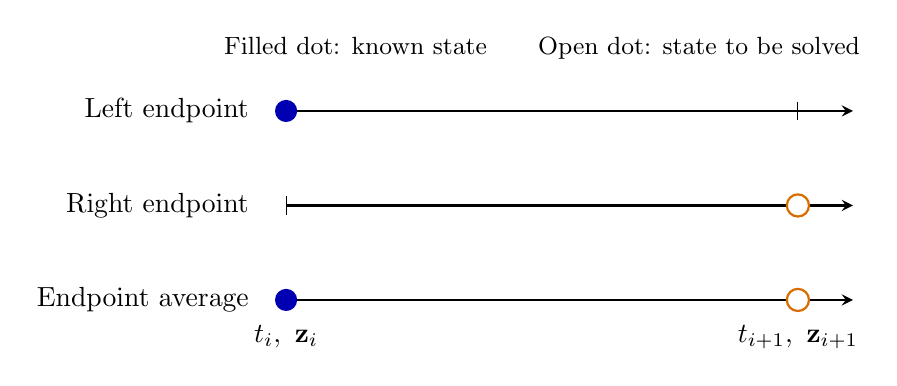
\begin{tikzpicture}[>=stealth,font=\normalsize]
\foreach \yy/\title in {2.4/{Left endpoint},1.2/{Right endpoint},0/{Endpoint average}}{
 \node[anchor=east]at(-.35,\yy){\title};
 \draw[->,thick](0,\yy)--(7.2,\yy);
 \draw(0,\yy+.12)--(0,\yy-.12);\draw(6.5,\yy+.12)--(6.5,\yy-.12);}
\fill[blue!70!black](0,2.4)circle(4pt);
\draw[orange!85!black,thick,fill=white](6.5,1.2)circle(4pt);
\fill[blue!70!black](0,0)circle(4pt);\draw[orange!85!black,thick,fill=white](6.5,0)circle(4pt);
\node[below]at(0,-.2){$t_i,\ \mathbf z_i$};\node[below]at(6.5,-.2){$t_{i+1},\ \mathbf z_{i+1}$};
\node[font=\small,align=center]at(3.25,3.2){Filled dot: known state\qquad Open dot: state to be solved};
\end{tikzpicture}
